\chapter{Reactive Swing Control for Trip Avoidance}\label{sec:trip_avoidance}
\graphicspath{{chapters/trip_avoidance/figures/}}

\emph{Material in this section based on}
\citet{gordon2019online}\cite{gordon2019online} \emph{and}
\citet{thatte2019realtime}\cite{thatte2019realtime} \linebreak

The experimental results from \cref{sec:nm_vs_imp}, in which we compared
neuromuscular and impedance control, revealed that trips during swing were one
of the most common causes for falls (\cref{tab:treadmill_exp_fall_reasons}). In
this chapter we explore two potential methods for avoiding swing trips. The
first focuses on avoidance of obstacles during gait through online learning of
classifiers that can recognize the user's obstacle avoidance intent. In the
second, we directly address the trips during normal walking that were observed
in \cref{sec:nm_vs_imp} by planning swing trajectories that use an estimate of
the user's hip height and orientation to avoid premature ground contact.

\section{Classification Approach Introduction}\label{sec:swing_control_class}

\begin{figure*}[t]
\centering
\includegraphics[width=\textwidth]{avoid_frames}
\caption{a)~Utilizing minimum jerk trajectories during swing does not allow for
appropriate adaptation of swing trajectories to enable obstacle avoidance.
b)~Our adaptive system learns online to detect the presence of an obstacle from
the amputee's late stance/early swing movements. Once detected, the controller
modifies the trajectories of the knee and ankle to achieve improved obstacle
clearance.}
\label{fig:avoid_frames}
\end{figure*}

Avoiding obstacles on the ground is a necessity for maintaining safety while
performing a variety of locomotion tasks. This behavior requires anticipation of
an obstacle and active leg control strategies to avoid it \citep{patla1995role}.
Transfemoral amputees, however, have a compromised ability to negotiate
obstacles, as shown in \Cref{fig:avoid_frames}, as current prosthesis technology
relies on mechanically passive knees that necessitate significant compensation
at the hip in order to replicate able-bodied trip recovery strategies
\citep{shirota2015transfemoral}. Compromised ability to avoid and recover from
trips may contribute to the large number of falls that leg amputees suffer. For
instance, 58\% of unilateral amputees reported a fall within a year
\citep{kulkarni1996falls}. Moreover, the fear of falling can cause amputees to
avoid activity, leading to further deterioration of their physical condition
\citep{miller2001prevalence}.

An increasing availability of powered prostheses in research labs provides the
opportunity to study active obstacle avoidance strategies in prosthetics,
although so far only a limited number of studies exist on this topic. These
studies focus on detecting and classifying the correct response strategy after
the amputee has tripped. For example, \citet{lawson2010stumble} developed a
classifier that uses fast Fourier transform and the root mean square of
accelerometer data as features to classify stumbles and recovery strategies,
respectively. \citet{zhang2011towards} found that adding EMG signals from the
residual limb to accelerometer data can help reduce false positives for stumble
and strategy detection. Finally, \citet{shirota2014recovery} identified the
optimal sliding window lengths and increments for feature calculation for trip
detection and strategy selection classifiers. While detecting and classifying
trip recovery strategies after their occurrence is a necessary step towards
obstacle avoidance, it does not provide a proactive prosthesis control strategy
that prevents obstacle encounters in the first place.

Another major drawback of the previous studies is that they train and test 
classifiers offline. However, a deployed trip classifier needs to function
online and deal with temporal adaptation of the learner and amputee. The
adaptation is required as the obstacle avoidance behavior triggered by a trip
classifier alters the amputee's movements and, therefore, the data used to train
the classifier. Consequently, trip classifiers trained offline may be
ineffective due to a mismatch of training and testing data. In
\cref{sec:back_high_level_control} we reviewed high-level classifiers that
detect transitions between gait modes such as standing, level ground walking,
and stair/ramp ascent/descent. In that setting, classification approaches often
run into a similar problem of training and testing data mismatch.
\citet{spanias2018online} provides a method of rectifying this data distribution
mismatch.

Here we present the first pilot study that combines online learning and
proactive control of a powered transfemoral prosthesis to implement obstacle
avoidance in amputee locomotion. The obstacle avoidance system uses early-swing
measurements of the residual limb angle, angular velocity, and linear
acceleration to recognize in-process obstacle avoidance attempts. To address the
online learning aspect of this system, we adapted the method proposed by
\citet{spanias2018online} for online learning of gait mode classification. We
also changed the existing swing leg behavior of the prosthesis to facilitate
obstacle avoidance. This change includes a regression to predict the appropriate
degree of knee and ankle flexion given the user's previous obstacle response
motions. Finally, we evaluated the system behavior in trials with both
non-amputee and amputee subjects.

\section{Classification Approach Methods}
\subsection{Forward-Backward Classifier}
In order to learn to classify trips online with minimal hand-labeling of data,
we rely primarily on the forward-backwards classifier approach first proposed by
\citet{spanias2018online} for the purpose of classifying different modes of gait
such as level ground walking, standing, and stair climbing. In their work, a
\emph{forward classifier} predicts the next step's gait mode using data in a
window shortly before the transition. In parallel, a \emph{backward classifier}
labels completed steps with their correct gait mode in hindsight. Because the
backwards classifier has access to features from the completed step, it can
achieve accurate labels with a small amount of hand-annotated data. Once
trained, the backwards classifier can provide labels for training the forward
classifier, obviating the need for further hand-labeling of steps. 

In our work, the forward classifier predicts, shortly after toe-off, if the
upcoming swing will require obstacle avoidance or not. For this purpose, we use
a linear support vector machine and features of the residual limb motion in the
last \unit[210]{ms} of stance and first \unit[90]{ms} of the swing phase.
Because user behavior changes over time in response to changes in prosthesis
obstacle avoidance behavior, we retrain the forward support vector machine every
ten steps using labels from the backward classifier. 

The backward classifier is another linear support vector machine, trained once
for each user, which uses features extracted from the entire swing phase to
label a step as an avoidance attempt after the fact. To train the backwards
classifier we hand label obstacle avoidance attempts and normal steps for
roughly ten obstacles. \Cref{fig:fwd_back} provides an overview of this system.

\begin{figure}[tb]
    \centerline{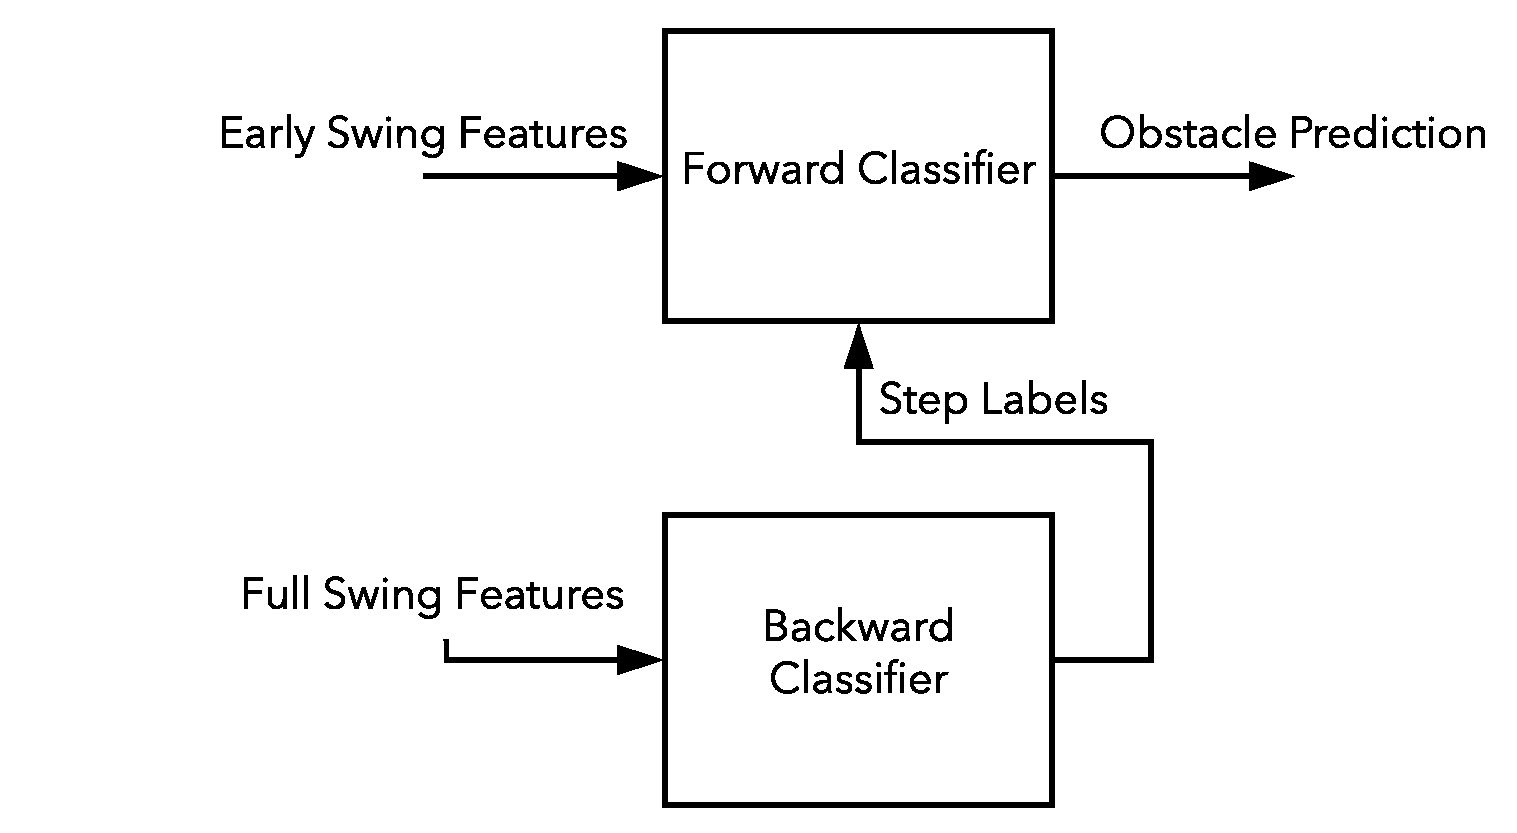
\includegraphics[width=\columnwidth]{Forward-Backward_Block_Diagram}}
    \caption[Forward-Backward Classifier Overview]{Forward-Backward Classifier
    Overview. The backwards classifier uses features from the entire swing to
    provide training class labels to a forwards classifier. The forwards
    classifier uses features from late stance and early swing in order to
    predict if an upcoming swing will be an obstacle avoidance
    attempt.}\label{fig:fwd_back}
\end{figure}

\subsection{Target Knee Angle Regression}

A prosthesis user will not always encounter obstacles of the same height. As the
obstacle avoidance response can be disruptive to the user, it is desirable to
give the user control over the magnitude of the prosthesis response. We seek to
achieve this functionality by using the normalized backward classifier score as
a metric for the difficulty of avoiding an obstacle. We then implement a simple
linear feedback law that assigns higher target flexion knee angles to obstacle
avoidance attempts that are more difficult according to this metric.
\Cref{fig:knee_reg} outlines this feedback mechanism, which has the form
\begin{align}
    \theta_{n+1}^{tgt} &= \theta_{n}^{tgt} - k_\tn{decay}(\theta_{n}^{tgt} 
        - \theta_\tn{min})     + k_\tn{score} \hat{\xi},\label{eq:tgt_angle}\\
    \hat{\xi} &= \frac{\xi - \xi_{10^\tn{th} \ \tn{percentile}}}{
        \xi_{90^\tn{th} \ \tn{percentile}} - \xi_{10^\tn{th} \ \tn{percentile}}},
        \label{eq:score_norm}
\end{align}
where $\theta_\tn{tgt}$ is the current target angle for a given set of features,
$n$ is the current time step, $k_\tn{decay}$ is a gain that prevents continual
target angle growth by decaying target angles towards $\theta_\tn{min}$, and
$k_\tn{score}$ is a gain on the normalized class score, $\hat{\xi}$. The system
shifts class scores, $\xi$, so that scores below the $10^\tn{th}$ percentile of
tripped step scores result in a reduction of the target knee angle. Furthermore,
the system normalizes the scores by $\xi_{90^\tn{th} \ \tn{percentile}} -
\xi_{10^\tn{th} \ \tn{percentile}}$ so that the gain $k_\tn{score}$ has a
predictable effect across subjects whose score ranges vary. 

The system fits the target knee angles with a linear support vector regression.
Every time the trip avoidance triggers, it appends an additional target angle,
specified by \cref{eq:tgt_angle}, to a training data set. The system retrains
the regression using this data set every ten trip-avoidance steps.

\begin{figure}[tb]
    \centerline{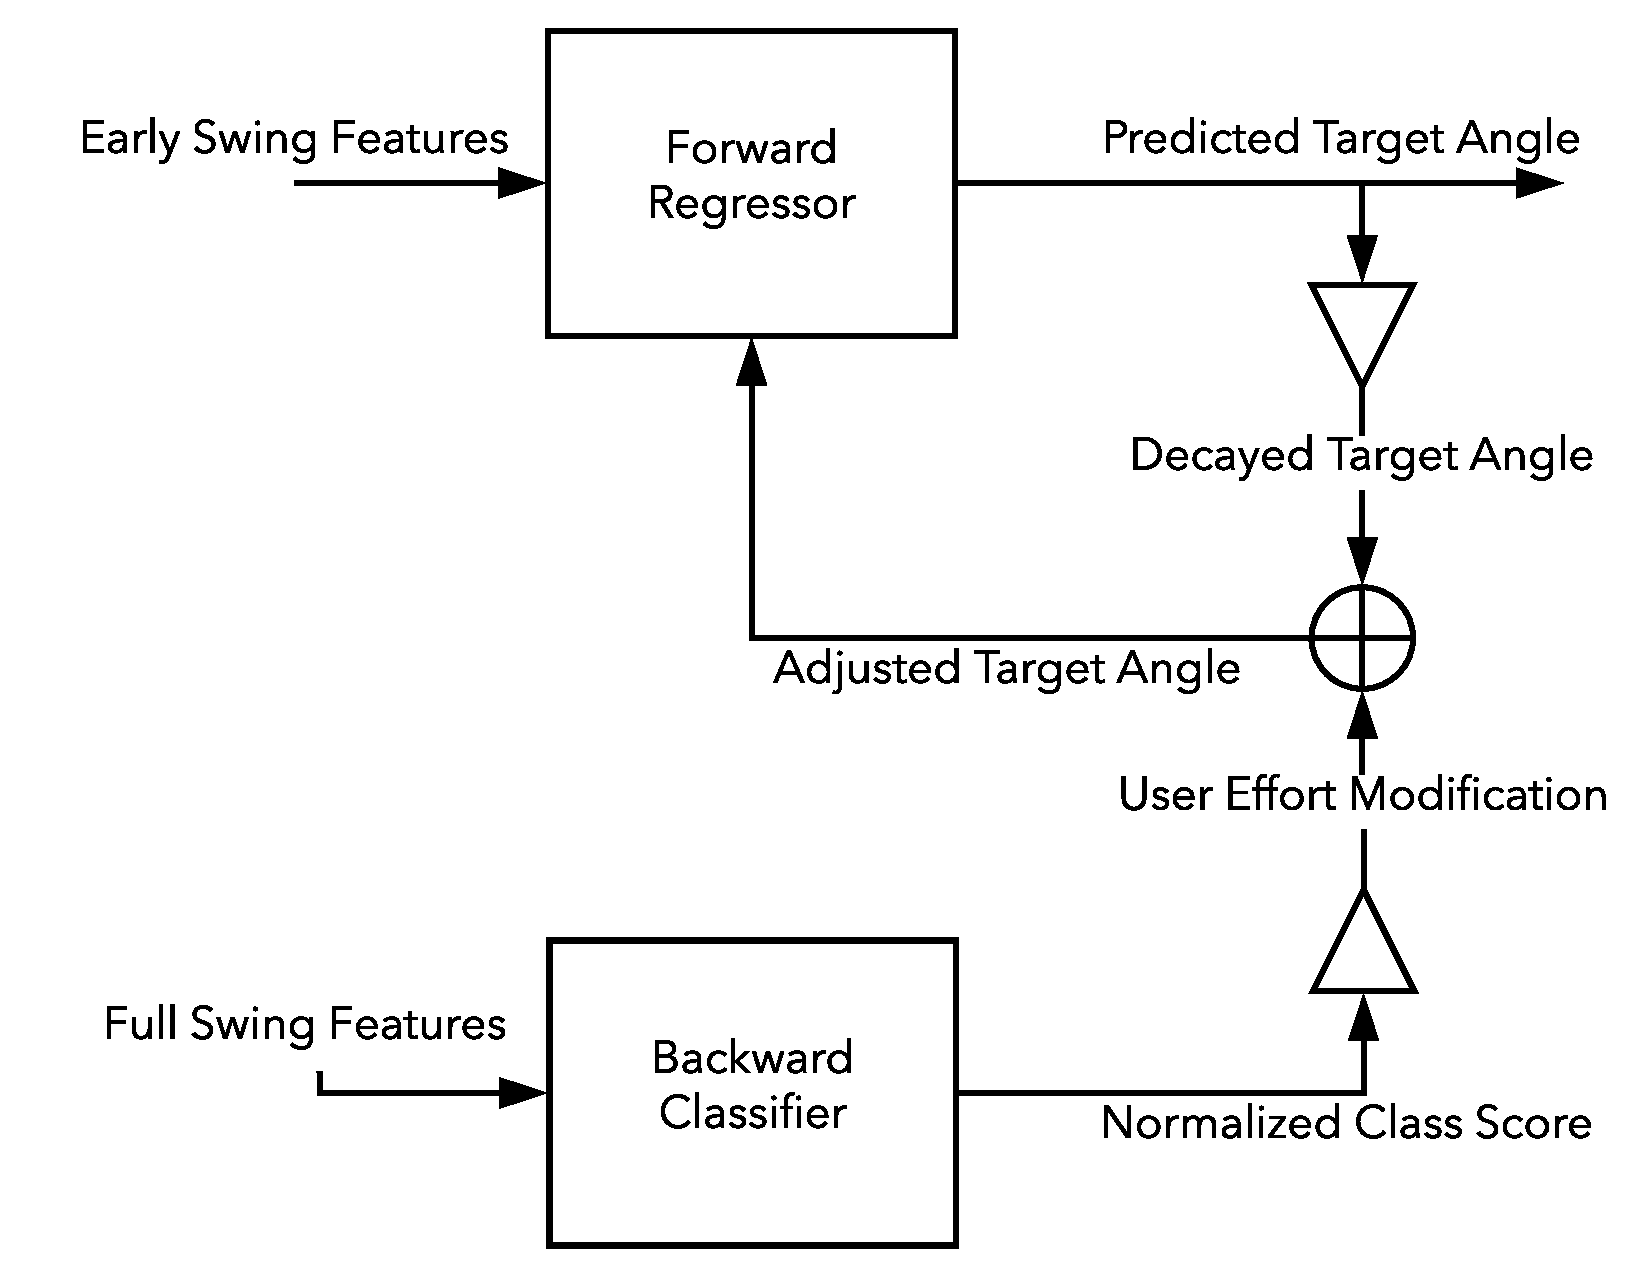
\includegraphics[width=\linewidth]{Regression_Block_Diagram}}
    \caption[Knee Angle Regression Feedback]{Knee Angle Regression Feedback. In
    order to enable volitional control of the knee and ankle flexion angles to
    allow users to achieve greater flexion angles for larger obstacles, we
    implement a feedback system that uses the backwards classifier class score
    to quantify obstacle difficulty. After each step, the system increases the
    desired target angle for that step's forward features proportionally to the
    normalized back classifier score. We also decay the current desired target
    angle for those features to prevent continual growth of the target angle.
    The regression is retrained every ten avoidance
    attempts.}\label{fig:knee_reg}
\end{figure}

\subsection{Feature Extraction}
For the forwards and backwards classifiers, as well as the target knee angle
regression, we use features of the thigh angle, angular velocity, and linear
accelerations in a time window. Specifically, we use the mean, standard
deviation, minimum value, and maximum value of each signal. For forward
classification and regression the time window begins \unit[210]{ms} before
toe-off and ends \unit[90]{ms} after toe-off, while for the backward
classification we use a window consisting of the entire swing phase between
toe-off and heel strike.

\subsection{Trajectory Planning}

To generate the knee and ankle motions for unperturbed swing, we follow the
method proposed by \citet{lenzi2014speed} to generate and follow human-like
minimum jerk trajectories that start at the toe-off state of each joint (angle,
angular velocity, and angular acceleration), go to a target flexion state, and
then extend to desired final angles at the estimated heel strike time. We
estimate the swing period to be $65\%$ of the stance period.

When the forward classifier triggers an obstacle avoidance attempt, we switch to
bang-bang trajectories for the knee and ankle joints. These trajectories
maximize foot clearance while respecting joint angle, velocity, and acceleration
limits. The bang-bang trajectories achieve desired flexion angles as quickly as
possible and then extend as late as possible such that they achieve extension
before the predicted heel strike time. The trajectory planner uses the target
knee angle regression to determine the appropriate peak angle for the knee
trajectory, while the ankle trajectory's target flexion angle is a linear
function of the knee's target angle. The knee trajectory's peak flexion angle is
constrained to lie within 65 and 90 degrees while the peak ankle flexion is
constrained within 5 and 15 degrees. Examples showing the minimum jerk swing
trajectories and obstacle avoidance trajectories planned for large and small
obstacles are given in \cref{fig:avoid_trajs}.

\begin{figure}[tb]
\centerline{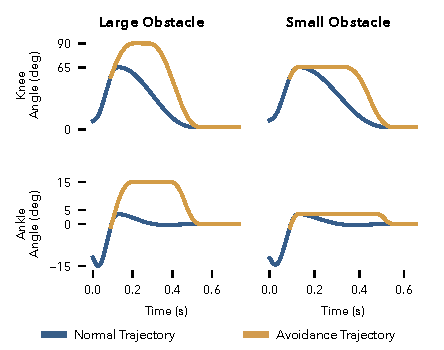
\includegraphics[width=\linewidth]{trajectories_legend}}
\caption[Bang-bang obstacle avoidance and minimum jerk swing
trajectories]{Bang-bang obstacle avoidance trajectories (yellow) vs normal
minimum jerk trajectories (blue) for the knee and ankle.}\label{fig:avoid_trajs}
\end{figure}

\subsection{Experimental Protocol}

We tested the ability of the proposed online learning system to accurately
classify trips and normal swings, help subjects avoid tripping on obstacles, and
modulate knee and ankle flexion appropriately for obstacles of different
heights. To evaluate these aspects of system performance, we conducted
experiments with the powered knee and ankle prosthesis previously described in
\cref{sec:pros_design}.

Two subjects, one non-amputee with prior experience using this prosthesis, and
one inexperienced amputee subject, performed walking trials with the obstacle
avoidance system enabled.  As subjects walked, an experimenter placed objects on
the treadmill belt in front of each subject's prosthetic leg, necessitating an
obstacle avoidance reaction. To obtain a baseline performance level for
non-reactive prosthetic swing control, we also performed obstacle avoidance
trials with the minimum jerk swing trajectories designed for undisturbed swing.
Before the online trials, the backwards classifier was trained for the
prosthesis user with 75 steps. The able bodied subject completed 446 total
steps, with 53 box avoidance steps, while the amputee completed 222 total steps,
with 40 box avoidance steps. The amputee subject performed trials in an ABBA
order, where A is minimum jerk control and B is the reactive control, in order
to average out potential learning effects. The amputee subject also had an
additional practice session the day prior to the box avoidance trials in which
he acclimated to walking with the powered prosthesis without obstacles.

\section{Classification Approach Results}

\subsection{Results}
\Cref{tab:able_class_perf,tab:amputee_class_perf} show the overall
classification accuracies, sensitivities, and specificities for the forward and
backwards classifiers for the able-bodied and amputee subjects respectively. The
forward and backwards classifiers for both subjects achieve high specificity
(the number of normal steps classified correctly) and accuracy $(>95\%)$. The
sensitivity, the percentage of true trips classified correctly, of the
classifiers for both subjects is substantially lower than the specificity or
accuracy. For the forward classifier, we see that because the model is trained
online, the sensitivity improves from the first half of the trial to the second
half, which explains some of the low overall sensitivity.

\begin{table}[htb]
\centering
\begin{tabular}{lccc}
    \multirow{2}{*}{Controller} & Classification & \multirow{2}{*}{Sensitivity} &
        \multirow{2}{*}{Specificity}\\
                                & Accuracy       &             &            \\
    \midrule
    Forward, $1^\tn{st}$ Half & 96\% \vsigstarone &  73\% \vsigstartwo & 99\%\\
    Forward, $2^\tn{nd}$ Half & 99\% ~            &  93\% ~            & 99\%\\
    Forward Overall           & 98\% ~            &  85\% \vsigstartwo & 99\%\\
    Backward                  & 99\% ~            & 100\% ~            & 99\%
\end{tabular}
\caption[Classifier Performance, Able-Bodied]{Classifier Performance
\protect\footnotemark, Able-Bodied Steps: 446, Avoidance Attempts:
53}\label{tab:able_class_perf}
\end{table}
\footnotetext{$\star \implies p<0.05$, $\star\star \implies p<0.01$,
$\star\negmedspace\star\negmedspace\star \implies p<0.001$, Chi-squared
test}

\begin{table}[htb]
\centering
\begin{tabular}{@{}lccc@{}}
    \multirow{2}{*}{Controller} & Classification & \multirow{2}{*}{Sensitivity} & 
        \multirow{2}{*}{Specificity} \\
               & Accuracy       &             &             \\
    \midrule
    Forward, $1^\tn{st}$ Half & 95\% & 80\% ~            & 98\%\\
    Forward, $2^\tn{nd}$ Half & 96\% & 85\% ~            & 98\%\\
    Forward Overall           & 95\% & 83\% \vsigstarone & 98\%\\
    Backward                  & 98\% & 90\% ~            & 99\%
\end{tabular}
\caption[Classifier Performance, Amputee]{Classifier Performance, Amputee, Total
Steps\protect\footnotemark[\value{footnote}]: 222, Avoidance Attempts:
40}\label{tab:amputee_class_perf}
\end{table}

Importantly, the ability of the forward classifier to correctly trigger the
bang-bang obstacle avoidance trajectories improves obstacle avoidance success
rates as shown in \cref{tab:success}. Both subjects were able to avoid
significantly more obstacles with the obstacle avoidance controller than with
the minimum jerk trajectory controller.

\begin{table}[htb]
\centering
\begin{tabular}{@{}lcc@{}}
    \multirow{2}{*}{Controller} & Able-Bodied  & Amputee \\
                                & Success Rate & Success Rate\\
    \midrule
    Minimum Jerk       & 37\% \vsigstarthree & 35\% \vsigstarthree\\
    Adaptive Bang-Bang & 89\% ~~             & 71\% ~~\\
\end{tabular}
\caption[Obstacle Avoidance Success Rates]{Obstacle Avoidance Success
Rates\protect\footnotemark[\value{footnote}]}\label{tab:success}
\end{table}

We also compared our online learning approach for obstacle avoidance to an
offline approach similar to that taken by \citet{lawson2010stumble,
zhang2011towards}, and \citet{shirota2015transfemoral}. To do this, we trained a
classifier offline using the first half of the amputee subject's bang-bang
control data and tested it on the second half of the data. \Cref{tab:offline}
shows that the classifier trained offline has trouble generalizing to the second
half of the data, as it performs significantly worse than the online-trained
model in terms of accuracy and sensitivity.

\begin{table}[ht]
\centering
{\begin{tabular}{@{}lccc@{}}
    Classifier & Classification Accuracy & Sensitivity         & Specificity \\
    \midrule
    Offline    & 89\% \vsigstarone       & 39\% \vsigstarthree & 100\% \\
    Online     & 95\% ~                  & 83\% ~              & 98\%\\
\end{tabular}}
\caption[Online and Offline Forward Classifier Performance, Amputee]{Online and
Offline Forward Classifier Performance,
Amputee\protect\footnotemark[\value{footnote}]}\label{tab:offline}
\end{table}

Finally, we examined the ability of the knee angle regression to choose a target
knee angle that is appropriate for the object size. The feedback law proposed in
\cref{eq:tgt_angle} assumes we can use the backwards classifier score as a
metric of obstacle difficulty. For the able-bodied subject, this assumption
seems warranted, as there is a strong relationship between the obstacle height
and the classifier score (\cref{fig:reg_and_height}a, $R^2 = 0.50$). However,
for the amputee subject, who was less experienced with walking with the powered
prosthesis, this relationship is less clear (\cref{fig:reg_and_height}B, $R^2 =
0.22$).

As shown in \cref{fig:reg_and_height}c\&d, our system is able to ensure that
high classification score steps, associated with high user effort, obtain larger
target flexion angles. This relationship led to noisy volitional control of the
knee flexion angle for the able-bodied subject (\cref{fig:reg_and_height}e) as
evidenced by the linear relationship between knee angle and obstacle height
$(R^2 = 0.31)$. However, for the amputee subject, there is no clear relationship
between the obstacle height and knee flexion angle (\cref{fig:reg_and_height}f,
$R^2 = 0.10$). 

\begin{figure*}[tb]
\centering
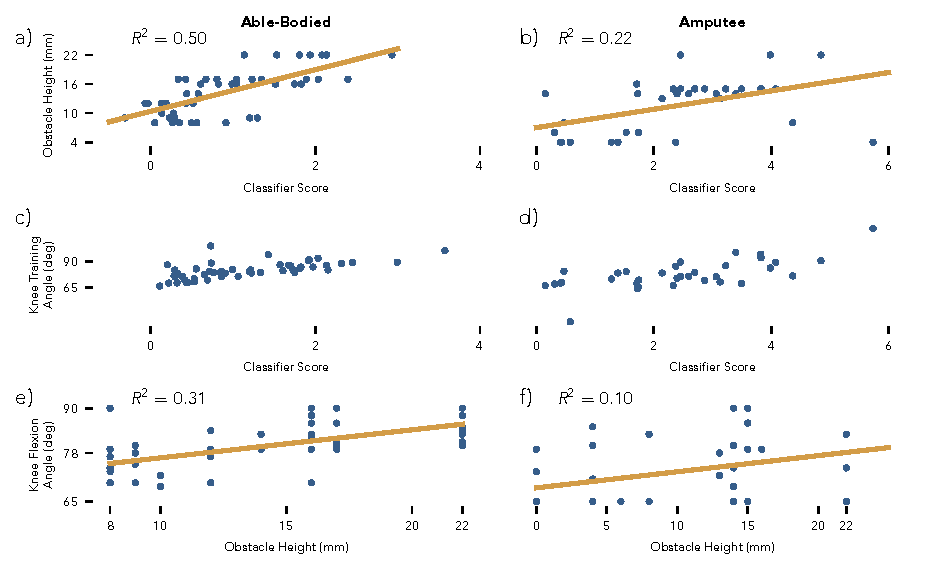
\includegraphics[width=\textwidth]{reg_and_height}
\caption{Obstacle height vs backwards classifier score for (a) the able-bodied
and (b) amputee subjects. The system uses the backwards classifier score as a
metric for obstacle avoidance difficulty. This score is used in a feedback loop
that forms the training set for the flexion target angle regression (c-d). With
this feedback system, the able bodied user (e) is able to achieve a degree of
volitional control over flexion angle as evidenced by the linear relationship
between knee flexion angle and obstacle height $(R^2=0.31)$. However, the
amputee (f) was not able to achieve meaningful control over the flexion of the
prosthesis $(R^2=0.10)$, possibly due to the decreased experience level of this
subject.}
\label{fig:reg_and_height}
\end{figure*}

\section{Classification Approach Discussion}

We developed an online learning system to help users of powered transfemoral
prostheses avoid obstacles. Our system uses information from an inertial
measurement unit during the late stance to early swing period to classify the
upcoming swing as either normal or a trip avoidance attempt. Unlike previous
work on obstacle negotiation for transfemoral prostheses
\citep{lawson2010stumble, zhang2011towards, shirota2014recovery}, our system
learns online on an actual transfemoral prostheses. We compared the
classification performance of our online system with a hypothetical offline
system using online trials to provide testing and training data for offline
analysis. This comparison showed that the online learning system provided an
improvement in sensitivity and accuracy to obstacle avoidance attempts. Both an
experienced, able-bodied subject and an inexperienced, amputee subject were able
to improve their obstacle avoidance success rates significantly. However, only
the experienced, able-bodied subject was able to achieve some level of
volitional control of the prosthesis flexion as a function of obstacle height.
                                  
There are several reasons why the amputee subject may not have been able to
achieve volitional control of prosthesis flexion. First, the amputee had far
less experience using the prosthesis than the able-bodied subject. Consequently,
even though both subjects were informed that trying harder to lift the leg over
bigger obstacles would likely lead to greater flexion once the prosthesis
learns, it is likely that only the first subject was able to incorporate and
implement this information. The amputee may have concentrated on more
rudimentary aspects of gait, as evidenced by his use of the handrails to walk,
whereas the able-bodied subject did not need to use the hand rails. Moreover,
the amputee's socket may have provided less control over the prosthesis than did
the intact subject's able-bodied adapter (shown in
\cref{fig:prosthesis_actual}).  Finally, we noted that the relationship between
joint flexion and obstacle height tended to oscillate over the course of our
trials. This may imply that the gains we used for the target knee angle
regression (\cref{eq:tgt_angle}) were too high.

Before settling on the specifics of the obstacle avoidance system presented
here, we also tested other options for its components. For example, we also
evaluated incorporating EMG signals from the non-prosthetic limb in our obstacle
avoidance classifier. Previous research showing that able-bodied subjects
utilize stance leg musculature to help raise the hip during obstacle avoidance
motivated this choice of EMG placement \citep{patla1995role}. However, as was
found by \citet{spanias2018online}, using EMG data along with mechanical data in
the forwards-backwards online learning algorithm did not seem to improve
classification accuracy, which is already high. This lack of improvement may
also result from a significant delay in our wireless EMG sensors (Delsys
Trigno). It is possible that a low-latency wired EMG sensor would be able to
improve classification performance or the performance of the target angle
regression.

We also tried using imitation learning techniques to model able-bodied
strategies for stepping over obstacles. Specifically, we employed maximum margin
inverse optimal control \citep{ratliff2007online} to learn, offline, cost
functions for the knee that explained obstacle avoidance trajectories. However,
when used online, the generated trajectories tended to diverge and produce
unexpected results because the initial toe-off state of the prosthesis did not
match those in the able-bodied data set. For the obstacle avoidance classifier,
we correct this sort of offline-online mismatch via the backwards classifier
that provides labels to train the forwards classifier online. It is less clear
how to update trajectories in hindsight as we never see the obstacle. For this
reason, we used bang-bang trajectories during obstacle avoidance, which maximize
the time the joints remain flexed.

In the future, this issue could be solved by incorporating a laser distance
sensor into the prosthesis. This sensor could enable precise measurement of the
ground and obstacle shape during the initial part of swing as the hip moves
forward. We could then use this information to explicitly plan knee and ankle
trajectories that will avoid the obstacle and the floor until the appropriate
touch down time. In the second half of this chapter, we present an initial step
in this direction in which we incorporate information from a laser distance
sensor to plan swing trajectories that help prevent trips on flat terrain.

There are several other limitations of the current study we should address in
future work as well. First, we only tested the algorithm with two subjects. More
subjects of varying skill levels are necessary to determine how applicable the
system is to a broader population. Additionally, a likely reason why the forward
classifier's sensitivity was relatively low, was that there were many more
normal steps than obstacle avoidance attempts in the training data set. This may
cause the SVM loss function's minimum to focus more heavily on classifying
normal steps correctly. Deploying this system on a commercial prosthesis, for
which trips are more rare, would exacerbate this issue. Therefore, future
development should investigate how to train a classifier given heavily
unbalanced class frequencies.

\section{Planning Approach Introduction}\label{sec:swing_control_planning}
Lower limb amputees using state of the art commercial prostheses face a number
of gait deficiencies that negatively impact their quality of
life~\citep{gauthier1999enabling}. Of acute significance among these
deficiencies are the increased risk of falling and the related injuries, which
can lead to amputees avoiding activity out of a fear
falling~\citep{miller2001prevalence}.  As falls and their avoidance are linked
to swing leg placement in locomotion, active swing control strategies could help
to substantially reduce the risk of falling. However, current swing controllers
of transfemoral prostheses do little to proactively minimize this risk. 

Existing swing phase control approaches for powered prostheses predominantly
seek to reproduce the average swing phase behavior of the human leg. Whether the
approach is based on trajectory planning~\citep{lenzi2014speed}, impedance
control~\citep{sup2009preliminary}, or phase-based
control~\citep{quintero2016preliminary}, they all treat the swing phase motion
as an ``open loop'' problem with respect to trip hazards, as none of the
approaches take the location of the heel and toe of the prosthetic foot with
respect to the ground explicitly into account. Therefore, current swing control
strategies neglect a clear advantage that robotic prostheses can have over their
passive counterparts: the ability to sense and act upon environmental
information. 

In this work, we develop a swing control strategy to reactively avoid trips with
powered transfemoral prostheses that uses visual information about the
environment and an estimate of the prosthesis configuration. Some previous
studies have explored incorporating visual feedback into the control of leg
prostheses. For example, \citet{scandaroli2009estimation} developed a state
estimator and controller that allowed the ankle joint of a prosthesis to conform
to the slope of the ground under the foot. To address the problem of terrain
recognition, \citet{zhang2011preliminary} developed a classifier using a LIDAR
and an IMU to discriminate between terrains such as flat ground and steps. More
recently, \citet{liu2016development} combined this terrain classifier with a
Bayesian intent classifier (based on \citep{du2012toward}) to develop an
environment-aware locomotion mode recognition system. In addition, RGBD sensors
have been explored as a source of rich environmental information for legged
assistance, including gait recognition \citep{massalin2017user} and stair
detection \citep{krausz2015depth,duan2018real}. However, none of these previous
studies have implemented a control strategy that uses environmental
information to reactively govern the motion of a powered prosthesis in
real-time. 

We present such a real-time reactive control of a powered prosthesis that
combines three building blocks. First, we use an extended Kalman filter (EKF)
that fuses measurements from an IMU, a LIDAR, and encoders on the prosthesis to
estimate the current pose of the prosthetic leg with respect to the ground.
Second, we predict likely future leg trajectories with sparse Gaussian process
models learned online during swing. Finally, we use the leg pose estimate and
trajectory predictions in a fast quadratic-program planner to reactively
generate in real time leg joint trajectories that avoid premature toe and heel
contact with the ground. To evaluate the proposed control, we compare our method
for trip avoidance to a standard non-reactive minimum-jerk trajectory planning
approach in a prosthesis walking experiment designed to elicit trips.

\section{Planning Approach Methods}
The trip avoidance control we propose involves (1) estimating the position and
orientation of the leg (\cref{sec:hip_kalman}), (2) predicting the future hip
angles and heights (\cref{sec:predict_gp}), and (3) planning corresponding knee
and ankle trajectories such that the heel and toe will not contact the ground
prematurely (\cref{sec:traj_plan}).

\subsection{Extended Kalman Filter for estimating Leg Position/Orientation}
\label{sec:hip_kalman}

To estimate the position and orientation of the leg, we employ an EKF that fuses
information from a LIDAR distance sensor (SICK OD1000), an IMU (YEI Technologies
3-Space sensor), and encoders on the prosthesis (Renishaw Resolute, Netzer
DS-25). The EKF filters the nonlinear, discrete-time dynamics given by
\begin{align}
    x_{t} = \begin{bmatrix} q_t \\ p_t \\ \dot{p}_t \end{bmatrix}
        &= \begin{bmatrix} f_\tn{gyro}(\omega_t) & 0 & 0 \\
            0 & I_{3\times3} & \Delta t  I_{3\times3}\\
            0 & 0 & I_{3\times3} \end{bmatrix} x_{t-1} \notag \\
        &\quad+ \begin{bmatrix} 0 \\ \frac{1}{2} \Delta t^2 I_{3\times3} \\ 
            \Delta t I_{3\times3} \end{bmatrix} 
        \begin{bmatrix} R_\tn{OI}(q_{t-1}) a_t - \begin{bmatrix} 0 \\ 0 \\ g 
            \end{bmatrix} \end{bmatrix} + w_t \label{eq:dynamics}\\
            &= f(x_{t-1}, u_t) + w_t  \notag ,
\end{align}
where $q$ is the quaternion orientation, $R_\tn{OI}$ and $p$ are the rotation
matrix and position of the IMU in inertial coordinates, $\omega$ is the angular
rate measured by the gyroscope, $f_\tn{gyro}$ integrates the gyroscope rate to
update the orientation, $a$ is the accelerometer measurement, $u_t =
\left[\omega_t, a_t \right]^T$, and $\Delta t$ is the integration time step
(\unit[1]{ms}). 

The dynamics are corrupted by process noise $w_t \sim \mathcal{N}(0, Q_t)$ due
to the inaccuracy of the IMU's measurement of the true acceleration and angular
velocity. Consequently, $Q_t$ is given by
\begin{align}
    Q_t = \left. \frac{\partial f}{\partial u} \right|_{x_{t-1}, u_t}
        \begin{bmatrix} \sigma_\omega^2 I_{3\times3} & 0 \\ 
            0 & \sigma_a^2 I_{3\times3} \end{bmatrix}
        \left. \frac{\partial f}{\partial u} \right|_{x_{t-1}, u_t}^T,
\end{align}
where $\sigma_\omega^2$ and $\sigma_a^2$ are the gyroscope and accelerometer
measurement variances, respectively.

\begin{marginfigure}
    \centering
    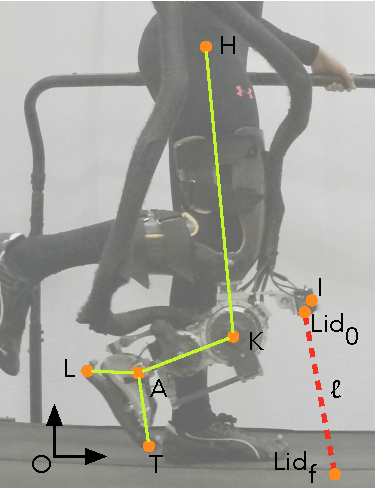
\includegraphics[width=\columnwidth]{kinematics}
    \caption{Kinematic model of the user and prosthesis used for state
    estimation and motion planning. The model includes the hip (H), knee (K),
    ankle (A), heel (L) and toe points (T). Additionally, the start ($Lid_0$)
    and end ($Lid_f$) points of the LIDAR beam (with length $\ell$) are
    indicated. The IMU is located at point $I$. Both the LIDAR and IMU are
    mounted to the thigh portion of the powered knee-and-ankle
    prosthesis.}\label{fig:kinematics}
\end{marginfigure}

To estimate the pose given our sensor measurements, we follow a standard EKF
procedure \citep{anderson1979optimal}, reviewed here for completeness. The EKF
state estimation process has two steps: First, we \emph{predict} the next state
distribution by forward-propagating the mean $\hat{x}_{t-1|t-1}$ and covariance
of the state estimate $\Sigma_{t-1|t-1}$ using the dynamics given by
\cref{eq:dynamics},
\begin{align}
    \hat{x}_{t|t-1} &= f(\hat{x}_{t-1|t-1}, u_t) \\
    \Sigma_{t|t-1} &= F_t \Sigma_{t-1|t-1} F_t^T + Q_t,
\end{align}
where $F_t = \left. \partial f / \partial x \right|_{\hat{x}_{t-1|t-1}}$.

Next, we incorporate information from noisy sensor observations to \emph{update}
the state estimate. To do this, we utilize a observation model given by $z_t =
h(x_t) + v_t$, where $v_t \sim \mathcal{N}\left(0, R \right)$, and the following
update equations:
\begin{align}
    K_t &= \Sigma_{t|t-1} H_t^T 
        {\left(H_t \Sigma_{t|t-1} H_t^T + R\right)}^{-1} \\
    \hat{x}_{t|t} &= \hat{x}_{t|t-1} + K_t \left(z_t - h(\hat{x}_{t|t-1}) \right) \\
    \Sigma_{t|t} &= \left(I - K_t H_t \right) \Sigma_{t|t-1}
\end{align}
where $z_t$ are the actual sensor measurements and $H_t = \left. \partial h /
\partial x \right|_{\hat{x}_{t-1|t}}$.

The observations in our EKF formulation use the kinematic model shown in
\cref{fig:kinematics}. We calibrate this model using ground truth data from a
VICON motion capture system. In our application we incorporate three
observations:
\begin{enumerate}
\item The expected acceleration vector points up in the global coordinate frame,
\begin{align} 
    h_1(x_t) &= {\left\{R_\tn{OI}(q) \right\}}_\textrm{row 3} \\
    z_1 &= a
\end{align}

\item The expected LIDAR measurement given the position of the IMU,
\begin{align}
    h_2(x_t) &= \left\{\ell : \left\{ p_\tn{OLID_f}\left(x_t, \ell \right)
        \right\}_\tn{row 3} = 0\right\} \\
    z_2 &= \ell_\tn{meas},
\end{align}
where $p_\tn{OLID_f}$, is the location of the laser beam endpoint represented in
the global coordinate system, $\ell = \lVert
\overrightarrow{\tn{LID_0}\tn{LID_f}} \rVert$ is the modeled laser beam length,
and $\ell_\tn{meas}$ is the actual measured LIDAR distance.

\item During stance, the toe point coincides with the origin (active
\unitfrac[200]{m}{s} after stance begins until toe-off)
\begin{align}
    h_3(x_t) &= p_\tn{OT}(x_t, \theta_\tn{k}, \theta_\tn{a}) \\
    z_3 &= {[0 \ 0 \ 0]}^T
\end{align}
where $p_\tn{OT}$ is the location of the toe in the inertial frame, and
$\theta_\tn{k}$ and $\theta_\tn{a}$ are the measured knee and ankle angles.
\end{enumerate}

The measurement noise for these observations is given by
\begin{align}
    R = \begin{bmatrix} \sigma_a^2 I_{3\times3} & 0 \\
        0 & \sigma_l^2 \end{bmatrix}
\end{align}
during swing and
\begin{align}
    R = \begin{bmatrix} \sigma_a^2 I_{3\times3} & 0 & 0 \\
        0 & \sigma_\ell^2 & 0 \\
        0 & 0 & \sigma_f^2 I_{3\times3} \end{bmatrix}
\end{align}
during stance. In these equations, $\sigma_a^2$ is the accelerometer variance,
$\sigma_\ell^2$ is the LIDAR measurement variance, and $\sigma_f^2$ is the foot
position variance.

To further improve the EKF's state estimate, we enforce a number of
constraints using the methods provided by \citet{gupta2007kalman}. Specifically,
we enforce three equality constraints:
\begin{enumerate}
\item First, we require that the quaternion has unit norm
\begin{align}
    1 = q_1^2 + q_2^2 + q_3^2 + q_4^2.
\end{align}

\item Second, we prevent the yaw component of the orientation $q$ from drifting.
To do this, we convert the $q$ to ZYX Euler angles and enforce $\phi_z = 0$, 
\begin{align}
    0 = \func{atan2}{2 (q_1 q_4 + q_2 q_3), 1 - 2 (q_3^2 + q_4^2)}.
\end{align}

\item Finally, during stance we further constrain the toe's $x$ and
$y$-coordinates to 0,
\begin{align}
    \begin{bmatrix} 0 \\ 0 \end{bmatrix} 
        &= {\left\{p_\tn{OT}(x_t, \theta_\tn{k}, \theta_\tn{a}) 
            \right\}}_\textrm{rows 1 and 2}.
\end{align}
\end{enumerate}

\noindent In addition, we use inequality constraints to ensure the toe and heel
do not penetrate the ground,
\begin{align}
    0 &\le {\left\{p_\tn{OT}(x_t, \theta_\tn{k}, \theta_\tn{a}) 
        \right\}}_\textrm{row 3} ,\\
    0 &\le {\left\{p_\tn{OL}(x_t, \theta_k, \theta_a) 
        \right\}}_\textrm{row 3}.
\end{align}

\noindent We enforce these constraints by solving the following quadratic
program after each update step,
\begin{align}
\hat{x}_{t|t}^\tn{proj} 
    &= {\argmin_x \left(x - \hat{x}_{t|t} \right)}^T \Sigma_{t|t}^{-1} 
        \left(x - \hat{x}_{t|t} \right),
\end{align}
such that
\begin{align}
    A_\tn{eq} x &= b_\tn{eq}, \\
    A_\tn{ineq} x &= b_\tn{ineq},
\end{align}
where $A_\tn{eq}$,  $b_\tn{eq}$, $A_\tn{ineq}$, and $b_\tn{ineq}$ are derived
from linearizing the equality and inequality constraints.

\begin{marginfigure}[-1in]
    \centering
    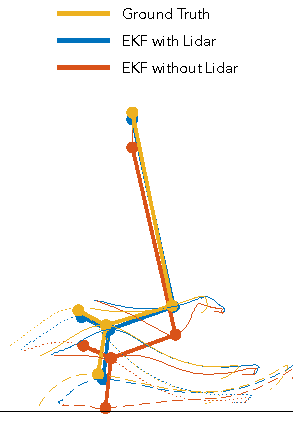
\includegraphics[width=\columnwidth]{ekf_fig}
    \caption{Trajectories of extended Kalman Filter (EKF) estimate of the
    position of the leg during swing (blue). Ground truth positions given by
    motion capture (yellow). EKF estimate without LIDAR information shown in
    red. Thick lines show the leg configuration at peak toe height during swing.
    Dotted lines indicate heel trajectories while dashed lines show the toe
    trajectories. Knee and ankle trajectories given by solid lines.}\label{fig:ekf}
\end{marginfigure}

To identify the appropriate parameters of the Kalman filter, we collected ground
truth training and testing kinematic data using a Vicon motion capture system
and optimized the parameters of the EKF to minimize the error of the kinematic
estimate. The parameters we optimized were the rotation of the LIDAR with
respect to the hip, the translation between the LIDAR and the IMU, and
$\sigma_\omega$, $\sigma_a$, $\sigma_\ell$, and $\sigma_f$. 

\Cref{fig:ekf} shows an example of the resulting EKF estimates of the hip, knee,
ankle, heel, and toe positions during swing (blue stick figure and traces)
compared to the ground truth obtained from the motion capture system (yellow)
and an EKF estimate without the LIDAR sensor information integrated (red). Over
the entire test data set, the root mean squared error of the estimated heel and
toe positions during swing is \unit[18.6]{mm} for the EKF with LIDAR
information. In contrast, the EKF without LIDAR information has an error of
\unit[46.7]{mm}. Thus, including the LIDAR sensor data reduces the error by
60\%.

\begin{figure}[t]
    \centering
    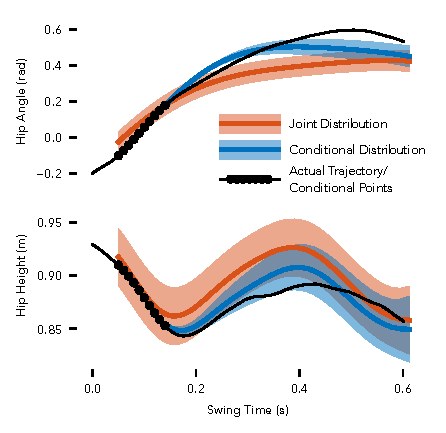
\includegraphics[width=\columnwidth]{gp_plots_w_legend}
    \caption{Example of hip angle and height trajectory predictions
    \unit[0.15]{s} into swing. The prediction algorithm uses the previous 10
    measured hip angles and heights (sampled at \unit[100]{Hz}, black dots)
    along with the learned joint distributions of hip angles/heights versus time
    (red) to obtain the conditional distributions of future hip angles/heights
    (blue). The planning algorithm uses the means of the conditional
    distributions to generate knee and ankle trajectories. The actual hip height
    and angle trajectories are shown in black.}
    \label{fig:gp_plots}
\end{figure}
\subsection{Gaussian Process Hip Trajectory Prediction}

\label{sec:predict_gp}
To predict the future hip angle and height trajectories, we train sparse
Gaussian process models using the FITC approximation \citep{snelson2007local}.
The sparse approximation ensures the computational complexity at test time is
independent of the training data set size, providing consistent real time
performance. Throughout the swing phase, the learned hip angle and height
distributions are conditioned on the swing trajectories completed so far to
predict the distribution of the future trajectories for the rest of the swing
(example shown in \cref{fig:gp_plots}). Our algorithm then uses the means of
these conditional distributions in the motion planning phase
(compare \cref{sec:traj_plan}). 

For example, to calculate the conditional mean of future hip angles, we first
compute the joint distribution of completed $(\theta_h^\tn{c})$ and future
$(\theta_h^\tn{f})$ hip angles,
\begin{align}
    \func{P}{\theta_h^\tn{c}, \theta_h^\tn{f}} &=
        \mathcal{N}\left(\mu_\tn{fitc}, \Sigma_\tn{fitc} 
            + K\left( t_\tn{joint}, t_\tn{joint} \right) \right) \\
    &= \mathcal{N}\left( 
        \begin{bmatrix} 
            \mu_\tn{c} \\ \mu_\tn{f} 
        \end{bmatrix},
        \begin{bmatrix} 
            \Sigma_{\tn{c},\tn{c}} & \Sigma_{\tn{c},\tn{f}} \\ 
            \Sigma_{\tn{f},\tn{c}} & \Sigma_{\tn{f},\tn{f}} 
        \end{bmatrix}
        \right),
\end{align}
where $\mu_\tn{fitc}$ and $\Sigma_\tn{fitc}$ are obtained from equation 11 in
\citep{snelson2007local} and $K\left( t_\tn{joint}, t_\tn{joint}\right)$ is an
additional noise term given by a rational quadratic kernel
\citep{rasmussen2004gaussian} that correlates the predicted angles across time,
which results in smooth predicted trajectories. The mean of the conditional
distribution $\func{P}{\theta_h^\tn{f}|\theta_h^\tn{c}}$ is then given by
\begin{align}
    \mu_\tn{f}^\tn{cond} = \mu_\tn{f} + \Sigma_{\tn{f},\tn{c}}
        \Sigma_{\tn{c},\tn{c}}^{-1}\left(\mu_\tn{c} - \theta_h^\tn{c} \right).
    \label{eq:gp_cond_mean}
\end{align}
As the inversion of $\Sigma_{\tn{c},\tn{c}}$ is the most computationally
expensive component of \cref{eq:gp_cond_mean}, we use at most the last 10 hip
angles and heights (sampled at \unit[100]{Hz}) when calculating the conditional
mean (compare \cref{fig:gp_plots}).

\subsection{Trajectory Planning Quadratic Program Formulation}
\label{sec:traj_plan}

\begin{pagefigure}
    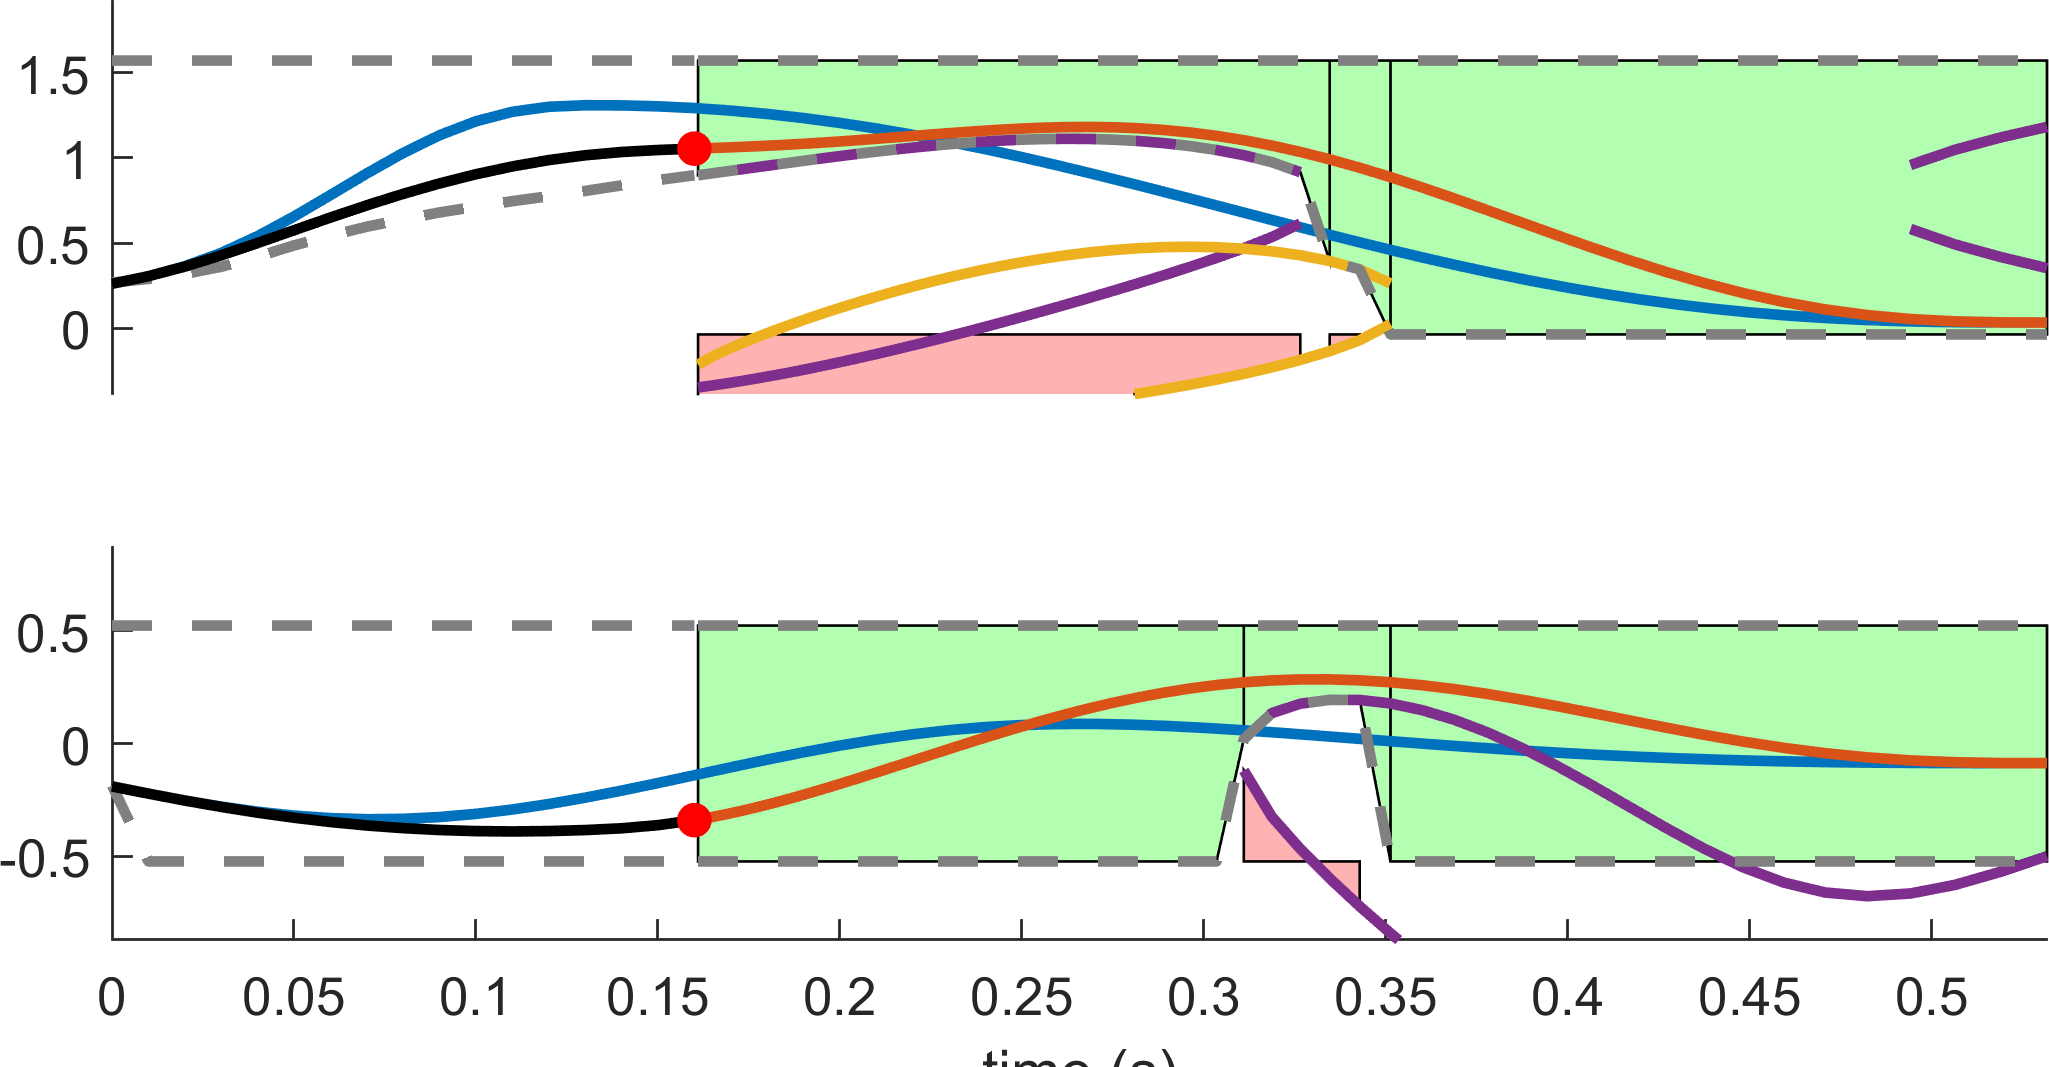
\includegraphics[width=\textwidth]{planning}
    \caption{Planning Algorithm Steps: Panels B and D
    show the generated knee and ankle trajectories respectively.  The planned
    trajectory (red) lies within the computed bounds (dashed gray).  In
    contrast, standard minimum jerk trajectories (blue) do not respect the
    bounds, thereby increasing the tripping hazard. Panels C and E show examples
    of inverse kinematics (IK) solutions for toe (purple) and heel (yellow)
    contact for the knee and ankle joints respectively. We use the IK solutions
    to generate bounded regions that the planned trajectory can safely traverse.
    We consider ground contact constraints for only the first half of the
    remaining swing duration after which we only consider joint angle
    constraints. We use Dijkstra's algorithm to select regions (green) that
    allow a path from the start point to the desired final point. Bounded
    regions that do not lie on the path are shown in red. Panel A shows the
    corresponding prosthesis motion.}\label{fig:planning}
\end{pagefigure}

To obtain reactive control of the prosthesis swing leg motion, we plan future
swing trajectories with a fast quadratic program (QP) operating at
\unit[100]{Hz}. The QP includes equality constraints, which ensure the
trajectories progress smoothly from the current position to the desired end
position, and inequality constraints, which avoid premature ground contact of
toe and heel of the prosthesis. Because in our formulation the QP can only solve
for one joint at a time, we first solve for the ankle trajectory assuming the
knee trajectory found in the previous time step, and then use this updated ankle
trajectory to solve for the new knee trajectory.

\Cref{fig:planning} provides more details of the actions of the trajectory
planner algorithm. For example, at a time of about \unit[150]{ms} into the swing
phase, the algorithm solves
\begin{align}
    \theta_\tn{k}^\textrm{toe bnd} 
        &= \left\{\theta_\tn{k} : \left\{p_\tn{OT}
            (\theta_\tn{h}, z_\tn{h}, \theta_\tn{k}, \theta_\tn{a})
            \right\}_\textrm{row 3} = 0 \right\} \\
    \theta_k^\textrm{heel bnd} 
        &= \left\{\theta_\tn{k} : \left\{p_\tn{OL}
            (\theta_\tn{h}, z_\tn{h}, \theta_\tn{k}, \theta_\tn{a})
            \right\}_\textrm{row 3} = 0 \right\}
\end{align}
at a set of sample times spanning the remaining swing trajectory to obtain a
planned knee trajectory (red trace in \cref{fig:planning}B).
Figures~\cref{fig:planning}C and E show the predicted inverse kinematics (IK)
solutions at characteristic points into the swing for the knee and ankle
respectively, with solutions leading to toe contact shown in purple and
solutions leading to heel contact shown in yellow. For each contact point, there
are typically two solutions, one lower bound, for which the joint angle cannot
cross from above, and one upper bound, for which the joint angle cannot cross
from below. 

Often, the valid leg configurations span disjointed regions in the configuration
space (green and red regions in \cref{fig:planning}B and D). Therefore, the
planner next identifies a valid sequence of regions for the trajectory to
traverse in a four step procedure.  First, the planner identifies critical
points along the predicted trajectory at which any bound activates or
deactivates. Second, at each critical point, the planner sorts the bound angles
from largest to smallest and iterates through them to define regions between
successive upper and lower bounds. Third, the planner defines a graph over the
regions with edge weights equal to the average squared angle minus the volume of
the child region. This cost favors a sequence of regions that are large and thus
safe to travel trough and avoids regions that require excessive joint flexion or
extension. Dijkstra's algorithm is then used to find a valid sequence of regions
that minimizes this cost~\citep{dijkstra1959note}. Finally, so that the
generated trajectories do not get too close to the identified bounds, a buffer
is added to the bounds. This buffer takes the form
\begin{align}
    \theta_\tn{buf} = \theta_\tn{buf}^0 \sin 
        \left(\pi \frac{t - t_0}{t_f - t_0} \right),
\end{align}
where $\theta_\tn{buf}^0$ is either \unit[5]{$^\circ$} or \unit[-5]{$^\circ$}
for lower and upper bounds respectively, $t$ is the future swing time, and $t_0$
and $t_f$ are the current and final swing times.

After identifying the bounded regions, the planner generates the trajectory for
a specific joint by solving a quadratic program. The trajectory of each joint is
represented by three, fifth-order polynomial splines,
\begin{align}
    \theta_1(t) &= a_{01} + a_{11} t + \cdots + a_{51} t^5 
        = [1 \ t \cdots t^5] a_1 \\ 
        T_0 &\le t < T_1 \\
    &\vdots \notag \\
    \theta_3(t) &= a_{03} + a_{13} t + \cdots + a_{53} t^5 
        = [1 \ t \cdots t^5] a_3 \\ 
     T_2 &\le t < T_F,
\end{align}
and solved for by the following QP,
\begin{align}
    a^* = \argmin_a \ \frac{1}{2} a^T (H_\theta + w H_{\dddot{\theta}}) a
    \label{eq:quadprog},
\end{align}
where $a = [a_1^T \ a_2^T \ a_3^T]^T$, $H_\theta$ and $H_{\dddot{\theta}}$
encode quadratic costs on angle and jerk respectively, and $w$ is a weight
parameter. The solution is subject to the inequality constraints
\begin{align}
    \theta(t) &\le \theta_\tn{max}(t), \ \forall t\\
    \theta(t) &\ge \theta_\tn{min}(t), \ \forall t\\
    \dot{\theta}(t) &\le \dot{\theta}_\tn{max}, \ \forall t\\
    \dot{\theta}(t) &\ge \dot{\theta}_\tn{min}, \ \forall t,
\end{align}
which ensure the trajectory lies within the identified bounds and respects
velocity limits, and to the equality constraints
\begin{align}
\theta(T_0) &= \theta_0 \\
\dot{\theta}(T_0) &= \dot{\theta}_0 \\
\ddot{\theta}(T_0) &= \ddot{\theta}_0 \\
\theta(T_F) &= \theta_F \\
\dot{\theta}(T_F) &= 0 \\
\ddot{\theta}(T_F) &= 0 \\
\theta_1(T_1) &= \theta_2(T_1) \\
\dot{\theta}_1(T_1) &= \dot{\theta}_2(T_1) \\
\ddot{\theta}_1(T_1) &= \ddot{\theta}_2(T_1) 
\label{eq:quadprog_last_constraint} \\
&\vdots \notag
\end{align}
which ensure the trajectory starts at the current and terminates at the desired
positions, velocities, and accelerations and that the splines join together
smoothly.  If the QP fails to find a trajectory that can satisfy the
constraints, the last found valid trajectory is reused for the next time step.
In addition, at the first iteration, the ankle trajectory planner uses the
output of the minimum jerk trajectory planner to solve the inverse kinematics
for the bounds. 

\subsection{Experimental Procedure}
We tested the ability of the proposed trip avoidance control to reduce the
incidence and severity of trips while walking with the powered transfemoral
prosthesis shown in \cref{fig:kinematics} To evaluate the performance of the
system, an able-bodied user walked with the prosthesis while attempting to
elicit trips by lowering the hip in swing. During the stance phase, the
prosthesis randomly decided to either use the proposed swing control or to use
standard minimum jerk trajectories that do not consider the tripping hazard. The
user was not aware of which controller would be used in the upcoming swing.  The
user completed a total of ten one minute walking trials.

We examined several outcomes for evaluating the control performance. First, we
examined the distribution of knee angles at the beginning of stance. Large knee
angles at the beginning of stance indicate premature landing due to toe-strike
instead of heel strike. Ideally, the landing angle is close to the desired final
angle of \unit[2]{degrees}. Second, we checked the integral of the ground
reaction force during swing. If this quantity is large, it indicates scuffing of
the toe on the ground. Finally, we examined the relationship between the hip and
toe heights during swing. If our controller is working as intended, the toe
height during swing should have a decreased sensitivity to the hip height.

\section{Planning Approach Results}

\begin{figure}[t]
    \centering
    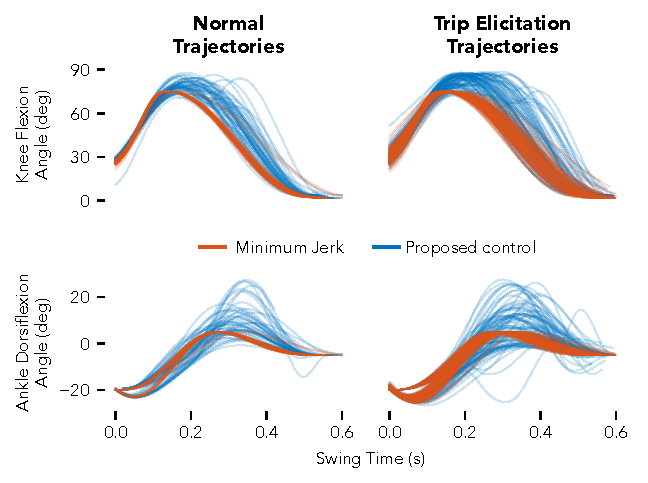
\includegraphics[width=\columnwidth]{trajectories_annotated}
    \caption{Knee and ankle trajectories produced during normal walking and
    while eliciting trips. To avoid tripping during trip elicitation trials,
    trajectories generated by the proposed approach often flex the knee to a
    greater degree and for longer before quickly extending at the end of swing.
    At the ankle joint we see overall greater variability in the generated
    trajectories during the trip elicitation condition versus normal walking.}
    \label{fig:trajectories}
\end{figure}

\Cref{fig:trajectories} shows the knee and ankle swing trajectories generated by
the proposed control (blue) and by a standard jerk minimization control (red)
during normal walking and trip elicitation. During undisturbed walking, the
trajectories produced by both control strategies are similar. However, the
proposed control strategy has a tendency to keep the knee flexed for longer and
then extends it faster towards the end of swing. In addition, in a few steps,
the proposed controller flexed the ankle significantly more than did the
standard minimum jerk control.  These trends are exaggerated during trip
elicitation. There are more knee trajectories in which the knee stays flexed for
longer, thereby creating more ground clearance. In addition, the ankle flexes
earlier, which will help to create more foot clearance when the hip is suddenly
lowered in early swing. 

We used video and audio recordings of the trials, as well as data from the
prosthesis, to manually classify trips as those swing trajectories that end with
toe strike or during which the foot scuffed on the ground. We find that over the
ten minutes of walking, the minimum jerk control produced 109 trips while the
proposed approach produced 35 trips, reducing the trip rate by 68\%.

\begin{figure}[t]
    \centering
    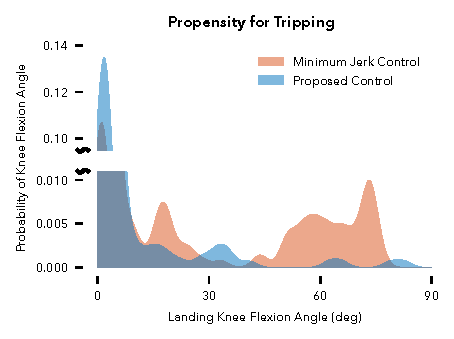
\includegraphics[width=\columnwidth]{prob_landing_angles}
    \caption{Kernel density estimate of the probability of various landing knee
    flexion angles with the proposed swing control (blue) and standard min-jerk
    swing control (red). Large landing knee angles indicate premature toe
    contact during swing.}
    \label{fig:p_landing_angle}
\end{figure}

To further examine the performance of the two control strategies, we used kernel
density estimates of the landing knee flexion angle, a measure of the propensity
for tripping, and integrated ground reaction force (GRF) during swing, a measure
of the propensity for foot scuffing. \Cref{fig:p_landing_angle} shows the
distributions of the landing angle of the prosthesis at the end of swing for the
proposed swing control (blue) and for the standard minimum jerk swing control
(red) during the trip elicitation condition. We observe the minimum jerk control
is much more likely to generate a swing trajectory that ends prematurely with a
large knee flexion angle, which is indicative of toe contact instead of heel
contact at the end of swing.  The distributions of the integrated GRFs suggests
the minimum jerk control produced a larger percentage of swings with high ground
reaction forces than the proposed control, indicating an increased frequency and
severity of toe scuffing during swing (\cref{fig:p_grf}). 
\begin{figure}[t]
    \centering
    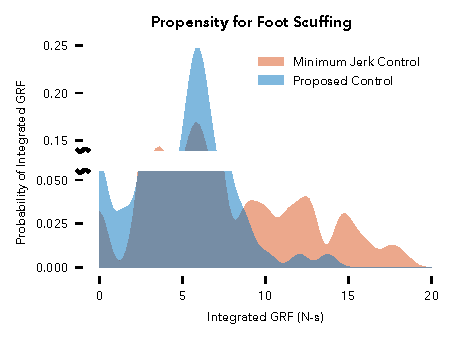
\includegraphics[width=\columnwidth]{prob_grf}
    \caption{Kernel density estimate of the probability of various integrated
    ground reaction force values for the proposed swing control (blue) and
    standard min-jerk swing control (red). Large integrated GRF during the swing
    phase is indicative of the toe scuffing on the ground.}
    \label{fig:p_grf}
\end{figure}

We can also ask the question, ``For steps during which the prosthesis used
trajectories generated by the proposed control, would the user have tripped had
the prosthesis used a minimum jerk trajectory?'' To answer this question, we can
use the kinematics model shown in \cref{fig:kinematics} along with ground truth
hip height and hip angle data captured via a motion capture system, to estimate
the location of the toe had the knee and ankle perfectly followed the desired
trajectories produced by each control scheme. This analysis predicts that the
prosthesis would have tripped or scuffed the toe on the ground during $22\%$ of
the steps if we had used the minimum jerk trajectory. In contrast, it predicts a
trip or scuff rate of $5\%$ had we perfectly followed the trajectories generated
by the proposed control.

\begin{figure}[t]
    \centering
    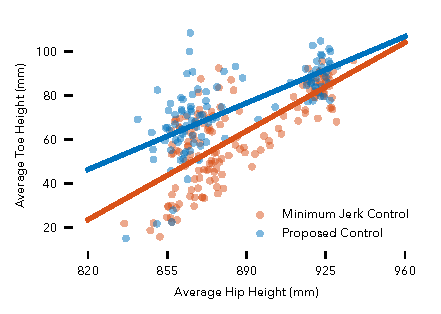
\includegraphics[width=\columnwidth]{toe_vs_hip_height}
    \caption{Average toe height vs average hip height for the proposed swing
    control (blue) and standard min-jerk swing control (red). The toe height
    during swing is less sensitive to the hip height when using the proposed
    swing control than when using the min-jerk swing control.}
    \label{fig:toe_vs_hip}
\end{figure}

Finally, \cref{fig:toe_vs_hip} shows the relationship between the average
toe and hip heights during swing for both control schemes. The toe height of the
prosthesis when controlled by the proposed control is less sensitive to
decreases in the hip height than it is when using the standard minimum jerk
control.

\section{Planning Approach Discussion}\label{sec:swing_control_planning_discuss}

We presented initial work toward a real-time reactive control of powered
prostheses to help amputees avoid tripping in the swing phase of gait. At any
time during swing, the proposed control uses a laser range finder and an
inertial measurement unit to estimate the current pose of the prosthesis,
predicts the future hip angle and height based on trained Gaussian process
models, and then plans new knee and ankle joint trajectories that ensure neither
the toe nor heel contacts the ground prematurely. Our results indicate the
proposed control approach can substantially reduce the incidence of trips and
reduce the severity and frequency of toe scuffing.

To the best of our knowledge, this work is the first demonstration of lower limb
prosthetic control that integrates perception feedback in real-time and that
proactively ameliorates the falling hazard amputees face. Previous research in
this area has largely focused on detecting stumbles \emph{after} they have
occurred. For example, \citet{lawson2010stumble} and \citet{shirota2014recovery}
have proposed classifiers that can detect trips during swing and predict whether
a lower or raising strategy should be used in response. Similarly,
\citet{zhang2011towards} have proposed a method that can detect stumbles and
classify them as trips during swing or slips during stance. However, these
previous studies have not proposed concrete control actions to preempt stumbles
or to properly react in the event that a stumble is detected. Our results
motivate further research into such proactive and reactive approaches, closing
the perception-action loop for improving gait robustness with robotic
prostheses.

Several avenues for future work exist. First, in our current study only one
able-bodied user tested the proposed control. Further experiments with amputee
subjects are needed to verify the system provides benefits to this population.
For instance, amputees accustomed to walking with passive prostheses show
significantly altered hip kinematics~\citep{jaegers1995prosthetic}, which could
affect the control behavior. However, the proposed control should be able to
properly adapt to these behavior differences, as the Gaussian process models are
trained for specific users. Second, although trips during swing are one of the
most common failure modes we encounter with our powered prostheses, these events
are still rare and many hours of normal walking are required to observe a
sufficient number of trips and compare controllers. As a result, we actively
induced trips by sudden drops in hip height during swing, which does not exactly
reflect the situations in which trips occur.  Specifically, trips can happen due
to subtle changes in leg kinematics, and it remains to be seen in experiments if
our approach can avoid trips in these more subtle situations.

At the implementation level, there is also room for further exploration. To keep
the  computational costs low, and due to ease of implementation in the
prosthesis' Simulink Real-Time\textsuperscript{TM} environment, we plan
trajectories using quadratic programs that iterate between finding solutions for
the ankle and knee joints.  While this iterative approach is fast when compared
to trajectory optimization methods that deal with multiple joints
simultaneously, the iterations occasionally get stuck when the planner for one
joint trajectory cannot find a solution based on the assumed fixed trajectory of
the other joint. Moreover, if a solution cannot be found, the current approach
simply reuses the last identified trajectory, rather than moving the trajectory
to be more safe, even if it cannot fully satisfy the bounds. It seems worthwhile
to investigate whether non-convex trajectory optimization methods such as CHOMP
\citep{ratliff2009chomp}, in which the bounds are represented as soft rather
than hard constraints, can help solve for the knee and ankle trajectories
simultaneously without sacrificing computational speed.

In addition, several technical simplifications can be considered to bring this
technology closer to commercialization. We used an accurate and expensive laser
distance sensor, eyeing future research in obstacle scanning and avoidance
capabilities. However, for simple ground plane avoidance, inexpensive infrared
distance sensors such as those used by \citet{scandaroli2009estimation} are
likely sufficient. It may also be possible to simplify the trajectory planning
phase by, for example, forgoing formal guarantees on satisfying bounds and
instead relying on heuristics to increase knee and ankle flexion and adjust
timing in response to decreased hip height during swing.

